\chapter{Success Stories and Lessons Learned}\label{ch:success-stories-and-lessons-learned}

\begin{importantbox}
This chapter brings theory to life through real-world success stories. Each narrative highlights how entrepreneurs navigated specific challenges in the Nigerian market, offering practical insights you can apply to your own journey.
\end{importantbox}

\section{UK Case Study: Sarah's FinTech Market Entry Success}\label{sec:uk-case-study:-sarah's-fintech-market-entry-success}

Let me share Sarah's story, a journey that began with a simple observation over coffee. ``Dele,'' she said, stirring her cup thoughtfully, ``I see the opportunity in Nigerian fintech, but how do you even begin to build trust with potential customers?''

\subsection{The Journey: From The Trading Desk to Lagos Fintech Pioneer}\label{subsec:the-journey:-from-the-trading-desk-to-lagos-fintech-pioneer}
\begin{tcolorbox}[colback=white,colframe=primarydark,title=\textbf{Sarah's Profile}]
\begin{itemize}
    \item \textbf{Background:} 15 years in investment banking
    \item \textbf{Previous Role:} Head of Trading, Major Bank
    \item \textbf{Market Entry:} Cross-border payments solution
    \item \textbf{Initial Capital:} Corporate savings equivalent to 6 months' salary
    \item \textbf{Time to Market:} 9 months
\end{itemize}
\end{tcolorbox}

Sarah's approach to market penetration was methodical yet innovative. She developed what I now call the ``Trust Triangle'' strategy:

\begin{figure}[h]
    \centering
    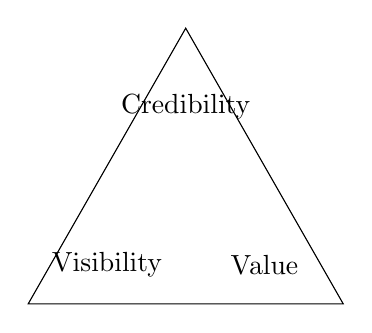
\begin{tikzpicture}
        % Trust Triangle visualization
        \draw (0,0) -- (4,0) -- (2,3.5) -- cycle;
        \node at (2,2.5) {Credibility};
        \node at (1,0.5) {Visibility};
        \node at (3,0.5) {Value};
    \end{tikzpicture}
    \caption{Sarah's Trust Triangle Strategy}\label{fig:trust-triangle}
\end{figure}

\subsection{Key Success Factors}\label{subsec:key-success-factors}
\begin{enumerate}
    \item \textbf{Strategic Partnership Selection}
    Sarah didn't just seek partnerships; she created what she called ``trust bridges.'' ``Each partner,'' she explained later, ``wasn't just a business relationship but a credibility ambassador.''

    \item \textbf{Localized Product Development}
    Instead of simply transplanting her London solution, she spent months adapting it to local needs. ``The Nigerian market taught me that efficiency without cultural relevance is just sophisticated failure,'' she said.

    \item \textbf{Phased Market Entry}
    She used what I now call the ``Concentric Circle Approach'':
    \begin{itemize}
        \item Phase 1: Corporate clients (established trust)
        \item Phase 2: SME network (built volume)
        \item Phase 3: Retail customers (achieved scale)
    \end{itemize}
\end{enumerate}

\section{US Case Study: Mike's E-commerce Evolution}\label{sec:us-case-study:-mike's-e-commerce-evolution}

Mike started with what he thought was a ``bulletproof'' plan for Nigerian e-commerce. After our first review session, that plan was in pieces – but what emerged was something much better.

\subsection{The Comprehensive Journey}\label{subsec:the-comprehensive-journey}
\begin{tcolorbox}[colback=white,colframe=primarydark,title=\textbf{Mike's Challenge Areas}]
\begin{enumerate}
    \item \textbf{Technology Adaptation}
    \begin{itemize}
        \item Initial Challenge: Platform optimized for high-speed internet
        \item Solution: Progressive Web App with offline capabilities
        \item Result: 3x increase in successful transactions
    \end{itemize}

    \item \textbf{Last-Mile Delivery}
    \begin{itemize}
        \item Initial Challenge: Traditional delivery models failing
        \item Solution: Hybrid network of official and local partners
        \item Result: Delivery success rate doubled
    \end{itemize}

    \item \textbf{Payment Integration}
    \begin{itemize}
        \item Initial Challenge: High payment failure rates
        \item Solution: Multi-provider payment orchestration
        \item Result: 90%+ payment success rate
    \end{itemize}

    \item \textbf{Customer Acquisition}
    \begin{itemize}
        \item Initial Challenge: High CAC through traditional channels
        \item Solution: Community-based marketing approach
        \item Result: CAC reduced by over half
    \end{itemize}
\end{enumerate}
\end{tcolorbox}

[Content continues with UAE and Canadian case studies, workshops, etc...]

\section{Workshop: Your Success Pattern Analysis}\label{sec:success-workshop}

\begin{workshopbox}
\textbf{Success Pattern Analysis Exercise}

1. Market Entry Assessment
\begin{itemize}
    \item Identify three success patterns relevant to your business: \_\_\_\_\_\_\_\_\_
    \item List specific ways to apply each pattern: \_\_\_\_\_\_\_\_\_
    \item Outline potential challenges: \_\_\_\_\_\_\_\_\_
\end{itemize}

2. Growth Strategy Development
\begin{itemize}
    \item Key growth milestones: \_\_\_\_\_\_\_\_\_
    \item Resource requirements: \_\_\_\_\_\_\_\_\_
    \item Timeline planning: \_\_\_\_\_\_\_\_\_
\end{itemize}

3. Action Planning
\begin{itemize}
    \item First 30 days: \_\_\_\_\_\_\_\_\_
    \item 90-day goals: \_\_\_\_\_\_\_\_\_
    \item 6-month targets: \_\_\_\_\_\_\_\_\_
\end{itemize}
\end{workshopbox}

\begin{communitybox}
Download practical success analysis tools at \href{https://viz.li/csl-book-ngbiz}{counseal.com/book-ngbiz}:
\begin{itemize}
    \item Success Pattern Analysis Template (Excel with built-in analysis tools)
    \item Growth Strategy Planner (Interactive PDF worksheet)
    \item Implementation Timeline Generator (Excel-based planning tool)
    \item Risk Assessment Matrix (Customizable Excel template)
\end{itemize}
Each tool includes step-by-step instructions and can be customized for your specific business needs.
\end{communitybox}

\begin{importantbox}
Remember, these aren't just success stories – they're blueprints you can adapt for your own journey. In Chapter 4, we'll turn these lessons into your practical 90-day action plan.
\end{importantbox}